\documentclass{ximera}

%\usepackage{todonotes}

\newcommand{\todo}{}

\usepackage{esint} % for \oiint
\ifxake%%https://math.meta.stackexchange.com/questions/9973/how-do-you-render-a-closed-surface-double-integral
\renewcommand{\oiint}{{\large\bigcirc}\kern-1.56em\iint}
\fi


\graphicspath{
  {./}
  {ximeraTutorial/}
  {basicPhilosophy/}
  {functionsOfSeveralVariables/}
  {normalVectors/}
  {lagrangeMultipliers/}
  {vectorFields/}
  {greensTheorem/}
  {shapeOfThingsToCome/}
  {dotProducts/}
  {partialDerivativesAndTheGradientVector/}
  {../productAndQuotientRules/exercises/}
  {../normalVectors/exercisesParametricPlots/}
  {../continuityOfFunctionsOfSeveralVariables/exercises/}
  {../partialDerivativesAndTheGradientVector/exercises/}
  {../directionalDerivativeAndChainRule/exercises/}
  {../commonCoordinates/exercisesCylindricalCoordinates/}
  {../commonCoordinates/exercisesSphericalCoordinates/}
  {../greensTheorem/exercisesCurlAndLineIntegrals/}
  {../greensTheorem/exercisesDivergenceAndLineIntegrals/}
  {../shapeOfThingsToCome/exercisesDivergenceTheorem/}
  {../greensTheorem/}
  {../shapeOfThingsToCome/}
  {../separableDifferentialEquations/exercises/}
  {vectorFields/}
}

\newcommand{\mooculus}{\textsf{\textbf{MOOC}\textnormal{\textsf{ULUS}}}}

\usepackage{tkz-euclide}
\usepackage{tikz}
\usepackage{tikz-cd}
\usetikzlibrary{arrows}
\tikzset{>=stealth,commutative diagrams/.cd,
  arrow style=tikz,diagrams={>=stealth}} %% cool arrow head
\tikzset{shorten <>/.style={ shorten >=#1, shorten <=#1 } } %% allows shorter vectors

\usetikzlibrary{backgrounds} %% for boxes around graphs
\usetikzlibrary{shapes,positioning}  %% Clouds and stars
\usetikzlibrary{matrix} %% for matrix
\usepgfplotslibrary{polar} %% for polar plots
\usepgfplotslibrary{fillbetween} %% to shade area between curves in TikZ
%\usetkzobj{all}
\usepackage[makeroom]{cancel} %% for strike outs
%\usepackage{mathtools} %% for pretty underbrace % Breaks Ximera
%\usepackage{multicol}
\usepackage{pgffor} %% required for integral for loops



%% http://tex.stackexchange.com/questions/66490/drawing-a-tikz-arc-specifying-the-center
%% Draws beach ball
\tikzset{pics/carc/.style args={#1:#2:#3}{code={\draw[pic actions] (#1:#3) arc(#1:#2:#3);}}}



\usepackage{array}
\setlength{\extrarowheight}{+.1cm}
\newdimen\digitwidth
\settowidth\digitwidth{9}
\def\divrule#1#2{
\noalign{\moveright#1\digitwidth
\vbox{\hrule width#2\digitwidth}}}




% \newcommand{\RR}{\mathbb R}
% \newcommand{\R}{\mathbb R}
% \newcommand{\N}{\mathbb N}
% \newcommand{\Z}{\mathbb Z}

\newcommand{\sagemath}{\textsf{SageMath}}


%\renewcommand{\d}{\,d\!}
%\renewcommand{\d}{\mathop{}\!d}
%\newcommand{\dd}[2][]{\frac{\d #1}{\d #2}}
%\newcommand{\pp}[2][]{\frac{\partial #1}{\partial #2}}
% \renewcommand{\l}{\ell}
%\newcommand{\ddx}{\frac{d}{\d x}}

% \newcommand{\zeroOverZero}{\ensuremath{\boldsymbol{\tfrac{0}{0}}}}
%\newcommand{\inftyOverInfty}{\ensuremath{\boldsymbol{\tfrac{\infty}{\infty}}}}
%\newcommand{\zeroOverInfty}{\ensuremath{\boldsymbol{\tfrac{0}{\infty}}}}
%\newcommand{\zeroTimesInfty}{\ensuremath{\small\boldsymbol{0\cdot \infty}}}
%\newcommand{\inftyMinusInfty}{\ensuremath{\small\boldsymbol{\infty - \infty}}}
%\newcommand{\oneToInfty}{\ensuremath{\boldsymbol{1^\infty}}}
%\newcommand{\zeroToZero}{\ensuremath{\boldsymbol{0^0}}}
%\newcommand{\inftyToZero}{\ensuremath{\boldsymbol{\infty^0}}}



% \newcommand{\numOverZero}{\ensuremath{\boldsymbol{\tfrac{\#}{0}}}}
% \newcommand{\dfn}{\textbf}
% \newcommand{\unit}{\,\mathrm}
% \newcommand{\unit}{\mathop{}\!\mathrm}
% \newcommand{\eval}[1]{\bigg[ #1 \bigg]}
% \newcommand{\seq}[1]{\left( #1 \right)}
% \renewcommand{\epsilon}{\varepsilon}
% \renewcommand{\phi}{\varphi}


% \renewcommand{\iff}{\Leftrightarrow}

% \DeclareMathOperator{\arccot}{arccot}
% \DeclareMathOperator{\arcsec}{arcsec}
% \DeclareMathOperator{\arccsc}{arccsc}
% \DeclareMathOperator{\si}{Si}
% \DeclareMathOperator{\scal}{scal}
% \DeclareMathOperator{\sign}{sign}


%% \newcommand{\tightoverset}[2]{% for arrow vec
%%   \mathop{#2}\limits^{\vbox to -.5ex{\kern-0.75ex\hbox{$#1$}\vss}}}
% \newcommand{\arrowvec}[1]{{\overset{\rightharpoonup}{#1}}}
% \renewcommand{\vec}[1]{\arrowvec{\mathbf{#1}}}
% \renewcommand{\vec}[1]{{\overset{\boldsymbol{\rightharpoonup}}{\mathbf{#1}}}}

% \newcommand{\point}[1]{\left(#1\right)} %this allows \vector{ to be changed to \vector{ with a quick find and replace
% \newcommand{\pt}[1]{\mathbf{#1}} %this allows \vec{ to be changed to \vec{ with a quick find and replace
% \newcommand{\Lim}[2]{\lim_{\point{#1} \to \point{#2}}} %Bart, I changed this to point since I want to use it.  It runs through both of the exercise and exerciseE files in limits section, which is why it was in each document to start with.

% \DeclareMathOperator{\proj}{\mathbf{proj}}
% \newcommand{\veci}{{\boldsymbol{\hat{\imath}}}}
% \newcommand{\vecj}{{\boldsymbol{\hat{\jmath}}}}
% \newcommand{\veck}{{\boldsymbol{\hat{k}}}}
% \newcommand{\vecl}{\vec{\boldsymbol{\l}}}
% \newcommand{\uvec}[1]{\mathbf{\hat{#1}}}
% \newcommand{\utan}{\mathbf{\hat{t}}}
% \newcommand{\unormal}{\mathbf{\hat{n}}}
% \newcommand{\ubinormal}{\mathbf{\hat{b}}}

% \newcommand{\dotp}{\bullet}
% \newcommand{\cross}{\boldsymbol\times}
% \newcommand{\grad}{\boldsymbol\nabla}
% \newcommand{\divergence}{\grad\dotp}
% \newcommand{\curl}{\grad\cross}
%\DeclareMathOperator{\divergence}{divergence}
%\DeclareMathOperator{\curl}[1]{\grad\cross #1}
% \newcommand{\lto}{\mathop{\longrightarrow\,}\limits}

% \renewcommand{\bar}{\overline}

\colorlet{textColor}{black}
\colorlet{background}{white}
\colorlet{penColor}{blue!50!black} % Color of a curve in a plot
\colorlet{penColor2}{red!50!black}% Color of a curve in a plot
\colorlet{penColor3}{red!50!blue} % Color of a curve in a plot
\colorlet{penColor4}{green!50!black} % Color of a curve in a plot
\colorlet{penColor5}{orange!80!black} % Color of a curve in a plot
\colorlet{penColor6}{yellow!70!black} % Color of a curve in a plot
\colorlet{fill1}{penColor!20} % Color of fill in a plot
\colorlet{fill2}{penColor2!20} % Color of fill in a plot
\colorlet{fillp}{fill1} % Color of positive area
\colorlet{filln}{penColor2!20} % Color of negative area
\colorlet{fill3}{penColor3!20} % Fill
\colorlet{fill4}{penColor4!20} % Fill
\colorlet{fill5}{penColor5!20} % Fill
\colorlet{gridColor}{gray!50} % Color of grid in a plot

\newcommand{\surfaceColor}{violet}
\newcommand{\surfaceColorTwo}{redyellow}
\newcommand{\sliceColor}{greenyellow}




\pgfmathdeclarefunction{gauss}{2}{% gives gaussian
  \pgfmathparse{1/(#2*sqrt(2*pi))*exp(-((x-#1)^2)/(2*#2^2))}%
}


%%%%%%%%%%%%%
%% Vectors
%%%%%%%%%%%%%

%% Simple horiz vectors
\renewcommand{\vector}[1]{\left\langle #1\right\rangle}


%% %% Complex Horiz Vectors with angle brackets
%% \makeatletter
%% \renewcommand{\vector}[2][ , ]{\left\langle%
%%   \def\nextitem{\def\nextitem{#1}}%
%%   \@for \el:=#2\do{\nextitem\el}\right\rangle%
%% }
%% \makeatother

%% %% Vertical Vectors
%% \def\vector#1{\begin{bmatrix}\vecListA#1,,\end{bmatrix}}
%% \def\vecListA#1,{\if,#1,\else #1\cr \expandafter \vecListA \fi}

%%%%%%%%%%%%%
%% End of vectors
%%%%%%%%%%%%%

%\newcommand{\fullwidth}{}
%\newcommand{\normalwidth}{}



%% makes a snazzy t-chart for evaluating functions
%\newenvironment{tchart}{\rowcolors{2}{}{background!90!textColor}\array}{\endarray}

%%This is to help with formatting on future title pages.
\newenvironment{sectionOutcomes}{}{}



%% Flowchart stuff
%\tikzstyle{startstop} = [rectangle, rounded corners, minimum width=3cm, minimum height=1cm,text centered, draw=black]
%\tikzstyle{question} = [rectangle, minimum width=3cm, minimum height=1cm, text centered, draw=black]
%\tikzstyle{decision} = [trapezium, trapezium left angle=70, trapezium right angle=110, minimum width=3cm, minimum height=1cm, text centered, draw=black]
%\tikzstyle{question} = [rectangle, rounded corners, minimum width=3cm, minimum height=1cm,text centered, draw=black]
%\tikzstyle{process} = [rectangle, minimum width=3cm, minimum height=1cm, text centered, draw=black]
%\tikzstyle{decision} = [trapezium, trapezium left angle=70, trapezium right angle=110, minimum width=3cm, minimum height=1cm, text centered, draw=black]


\title{Rational}

\begin{document}

\begin{abstract}
fractions of polynomials
\end{abstract}
\maketitle




Rational functions are fractions of polynomials


\begin{definition}\textbf{\textcolor{green!50!black}{Rational Functions}}

A rational function is any function that can be represented as a quotient of two polynomials 

\[   \frac{ a_n x^n + a_{n-1} x^{n-1} + \cdots + a_3 x^3 + a_2 x^2 + a_1 x + a_0  } { b_m x^m + b_{m-1} x^{m-1} + \cdots + b_3 x^3 + b_2 x^2 + b_1 x + b_0 }   \]



where the $a_k$ and $b_k$ are real numbers and $a_n \ne 0$ and $b_m \ne 0$.





\end{definition}




Again, we prefer polynomials in factored form.  Therefore, usually, our first step is to transform the formula for the rational function to look like



\[   \frac{ (x-r_n)(x-r_{n-1})  \cdots (x-r_2)(x-r_1)  } { (x-s_m)(x-s_{m-1})  \cdots (x-s_2)(x-s_1) }   \]




And, again, we will be able to obtain a product of exclusively linear factors with the addition of complex numbers.  With real numbers we can get these products to consist of a mixture of linear and irreducible quadratics.










\begin{example}


The graph of $y = H(w) = \frac{(w-1)}{(w+3) (w-4)} $


\begin{image}
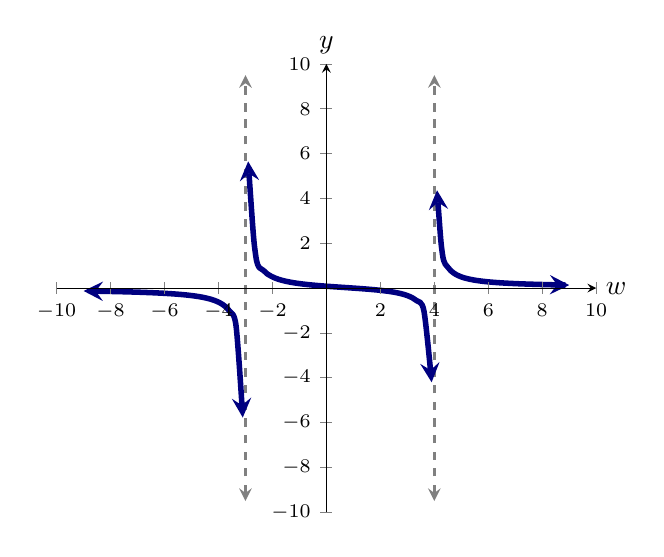
\begin{tikzpicture} 
  \begin{axis}[
            domain=-10:10, ymax=10, xmax=10, ymin=-10, xmin=-10,
            axis lines =center, xlabel=$w$, ylabel=$y$,
            ytick={-10,-8,-6,-4,-2,2,4,6,8,10},
            xtick={-10,-8,-6,-4,-2,2,4,6,8,10},
            ticklabel style={font=\scriptsize},
            every axis y label/.style={at=(current axis.above origin),anchor=south},
            every axis x label/.style={at=(current axis.right of origin),anchor=west},
            axis on top
          ]

          \addplot [line width=1, gray, dashed, domain=(-9.5:9.5),<->] ({-3},{x});
          \addplot [line width=1, gray, dashed, domain=(-9.5:9.5),<->] ({4},{x});

          \addplot [line width=2, penColor, smooth, domain=(-9:-3.1),<->] {(x-1)/((x+3)*(x-4))};
          \addplot [line width=2, penColor, smooth, domain=(-2.9:3.9),<->] {(x-1)/((x+3)*(x-4))};
          \addplot [line width=2, penColor, smooth, domain=(4.1:9),<->] {(x-1)/((x+3)*(x-4))};


  \end{axis}
\end{tikzpicture}
\end{image}

\end{example}








\begin{example}


The graph of $y = v(r) = \frac{(r-1)}{(r+3) (r-4)^2} $


\begin{image}
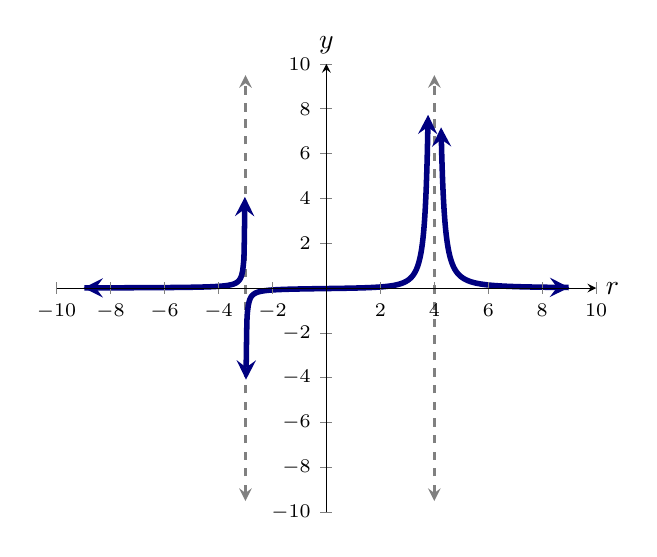
\begin{tikzpicture} 
  \begin{axis}[
            domain=-10:10, ymax=10, xmax=10, ymin=-10, xmin=-10,
            axis lines =center, xlabel=$r$, ylabel=$y$,
            ytick={-10,-8,-6,-4,-2,2,4,6,8,10},
            xtick={-10,-8,-6,-4,-2,2,4,6,8,10},
            ticklabel style={font=\scriptsize},
            every axis y label/.style={at=(current axis.above origin),anchor=south},
            every axis x label/.style={at=(current axis.right of origin),anchor=west},
            axis on top
          ]

          \addplot [line width=1, gray, dashed, domain=(-9.5:9.5),<->] ({-3},{x});
          \addplot [line width=1, gray, dashed, domain=(-9.5:9.5),<->] ({4},{x});

          \addplot [line width=2, penColor, smooth, samples=200, domain=(-9:-3.02),<->] {(x-1)/((x+3)*(x-4)^2)};
          \addplot [line width=2, penColor, smooth, samples=200, domain=(-2.98:3.77),<->] {(x-1)/((x+3)*(x-4)^2)};
          \addplot [line width=2, penColor, smooth, samples=200, domain=(4.25:9),<->] {(x-1)/((x+3)*(x-4)^2)};


  \end{axis}
\end{tikzpicture}
\end{image}

\end{example}








While polynomials only combined factors with positive integer powers, rational functions include factors with negative integer powers.


We can pull $H(w)$ apart to see these power-like functions.


\[    H(w) = \frac{(w-1)}{(w+3) (w-4)}  = \frac{4}{7} \cdot \frac{1}{w+3}  + \frac{3}{7} \cdot \frac{1}{w-4}    \]


Not strictly speaking power functions, but more like shifted power functions - in the denominator.









\subsection{Continuity}


Rational functions are continuous everywhere on their domain.  They have singularities at zeros of their denominators.  

Graphs of rational functions might have vertical asymptotes at these singularities, where the function grows (positively or negatively) without bound.  As we can see in the examples above, the sign of the function can switch across a singularity, or not.  This has to do with the power of the corresponding factor, which we will investigate later.













\begin{example}


The graph of $y = B(c) = \frac{(c-1)(c-5)}{5(c+3)} $


\begin{image}
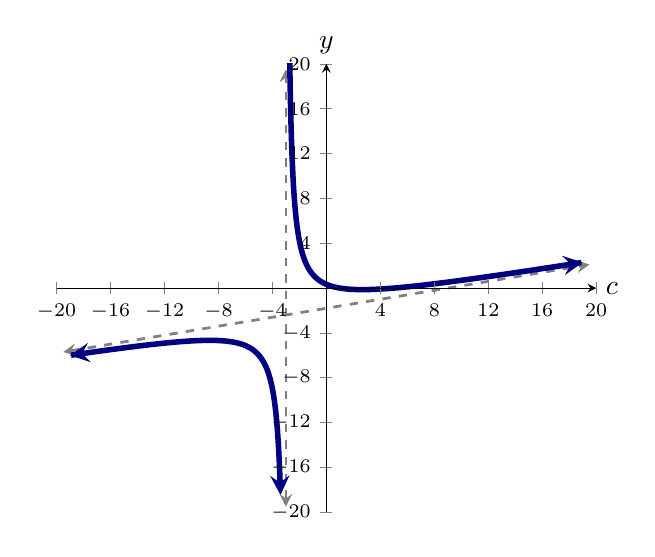
\begin{tikzpicture} 
  \begin{axis}[
            domain=-20:20, ymax=20, xmax=20, ymin=-20, xmin=-20,
            axis lines =center, xlabel=$c$, ylabel=$y$,
            ytick={-20,-16,-12,-8,-4,4,8,12,16,20},
            xtick={-20,-16,-12,-8,-4,4,8,12,16,20},
            ticklabel style={font=\scriptsize},
            every axis y label/.style={at=(current axis.above origin),anchor=south},
            every axis x label/.style={at=(current axis.right of origin),anchor=west},
            axis on top
          ]


          \addplot [line width=1, gray, dashed, domain=(-19.5:19.5),<->] ({-3},{x});
          \addplot [line width=1, gray, dashed, domain=(-19.5:19.5),<->] {0.2*x-1.8};


          \addplot [line width=2, penColor, smooth, samples=200, domain=(-19:-3.4),<->] {((x-1)*(x-5))/(5*(x+3))};
          \addplot [line width=2, penColor, smooth, samples=200, domain=(-2.9:19),<->] {((x-1)*(x-5))/(5*(x+3))};



  \end{axis}
\end{tikzpicture}
\end{image}

\end{example}




In addition to horizontal and vertical asymptotes, rational functions can have \textbf{oblique} asymptotes, which describe the end-behavior.












The graph of a rational function need not have an asymptote at a zero of the denominator.


\begin{example}


The graph of $y = h(t) = \frac{(t-1)(t-5)}{(t-5)(t+3)} $ \\

$5$ is a zero of the polynomial in the denominator.  However, $t=5$ is not an asymptote in the graph.


\begin{image}
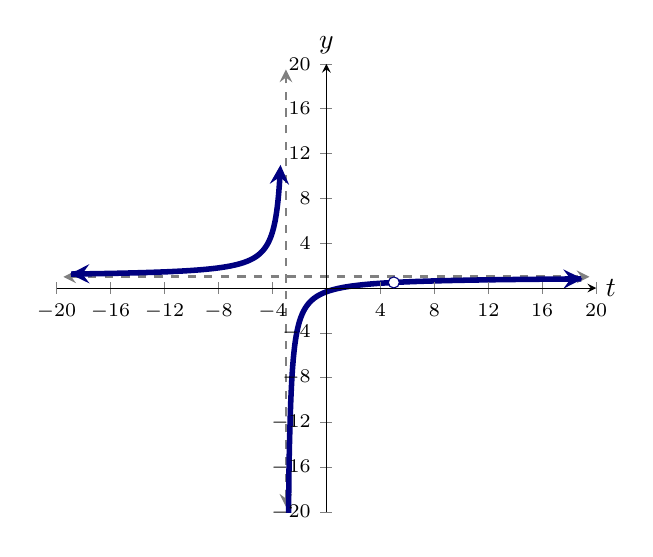
\begin{tikzpicture} 
  \begin{axis}[
            domain=-20:20, ymax=20, xmax=20, ymin=-20, xmin=-20,
            axis lines =center, xlabel=$t$, ylabel=$y$,
            ytick={-20,-16,-12,-8,-4,4,8,12,16,20},
            xtick={-20,-16,-12,-8,-4,4,8,12,16,20},
            ticklabel style={font=\scriptsize},
            every axis y label/.style={at=(current axis.above origin),anchor=south},
            every axis x label/.style={at=(current axis.right of origin),anchor=west},
            axis on top
          ]
 
          \addplot [line width=1, gray, dashed, domain=(-19.5:19.5),<->] ({-3},{x});
          \addplot [line width=1, gray, dashed, domain=(-19.5:19.5),<->] ({x},{1});

          \addplot [line width=2, penColor, smooth, samples=200, domain=(-19:-3.4),<->] {(x-1)/(x+3)};
          \addplot [line width=2, penColor, smooth, samples=200, domain=(-2.9:19),<->] {(x-1)/(x+3)};


          \addplot[color=penColor,fill=white,only marks,mark=*] coordinates{(5,0.5)}; 
                 

  \end{axis}
\end{tikzpicture}
\end{image}

\end{example}


This is because $5$ is also a zero of the polynomial in the numerator.


\[ y = h(t) = \frac{(t-1)(t-5)}{(t-5)(t+3)} = \frac{(t-1)}{(t+3)}  \, \text{ for } \,  t \ne 5  \]










\section*{End-Behavior}



The end-behavior of a rational function depends on the leading terms of the numerator and denominator.





\textbf{\textcolor{red!90!darkgray}{$\blacktriangleright$}} If $n > m$




\[   \lim\limits_{x \to \pm\infty}  \frac{ a_n x^n + a_{n-1} x^{n-1} + \cdots + a_3 x^3 + a_2 x^2 + a_1 x + a_0  } { b_m x^m + b_{m-1} x^{m-1} + \cdots + b_3 x^3 + b_2 x^2 + b_1 x + b_0 }   = \lim\limits_{x \to \pm\infty} \frac{ a_n x^n } { b_m x^m } = \pm \infty
\]











\textbf{\textcolor{red!90!darkgray}{$\blacktriangleright$}} If $n < m$




\[  \lim\limits_{x \to \pm\infty} \frac{ a_n x^n + a_{n-1} x^{n-1} + \cdots + a_3 x^3 + a_2 x^2 + a_1 x + a_0  } { b_m x^m + b_{m-1} x^{m-1} + \cdots + b_3 x^3 + b_2 x^2 + b_1 x + b_0 }   = \lim\limits_{x \to \pm\infty} \frac{ a_n x^n } { b_m x^m } = 0
\]











\textbf{\textcolor{red!90!darkgray}{$\blacktriangleright$}} If $n = m$




\[  \lim\limits_{x \to \pm\infty} \frac{ a_n x^n + a_{n-1} x^{n-1} + \cdots + a_3 x^3 + a_2 x^2 + a_1 x + a_0  } { b_m x^m + b_{m-1} x^{m-1} + \cdots + b_3 x^3 + b_2 x^2 + b_1 x + b_0 }   =  \lim\limits_{x \to \pm\infty} \frac{ a_n x^n } { b_m x^m } = \frac{ a_n} { b_m }
\]




























\begin{center}
\textbf{\textcolor{green!50!black}{ooooo=-=-=-=-=-=-=-=-=-=-=-=-=ooOoo=-=-=-=-=-=-=-=-=-=-=-=-=ooooo}} \\

more examples can be found by following this link\\ \link[More Examples of Elementary Functions]{https://ximera.osu.edu/csccmathematics/precalculus1/precalculus1/elementaryLibrary1/examples/exampleList}

\end{center}



\end{document}
